\chapter{Wyniki}

\section{Wprowadzenie}

Dla wszystkich, zaimplementowanych w poprzednim rozdziale algorytmów przeprowadzono testy pokazujące skuteczność ich działania na wybranych klasach grafów. Na początku przeprowadzono testy dla różnych kombinacji hiperparametrów algorytmu mrówkowego, w celu uzyskania najlepszego zestawu parametrów dla tego problemu, który będzie następnie wykorzystywany w dalszych rozważaniach. Następnie przedstawiono wyniki dla wybranych klas grafów:
\begin{itemize}
    \item grafy rzadkie
    \item grafy gęste
    \item drzewa
    \item grafy bezskalowe
\end{itemize}
Grafy każdej klasy wygenerowano z następującą liczbą wierzchołków: $[10, 20, 30, 40, 50]$, dla każdej liczby wierzchołków po 3 razy. Dla spójności, wszystkie algorytmy, tam gdzie to ma sens, testowano na tych samych wygenerowanych grafach. Dalej w tabeli zostaną przedstawione wyniki poglądowe jednego z trzech takich zestawów. 
Wszystkie średnie pomiary czasów w tabelach przedstawiono w sekundach. Pomiary dla każdego przypadku wykonywano pięciokrotnie w celu otrzymania wiarygodnego wyniku. Pomiary mierzono w nanosekundach z niepewnością pomiaru wynoszącą 100 nanosekund, wykorzystując funkcję \textit{time.perf\_counter\_ns()}. Dodatkowo dla każdej klasy przedstawiono wykresy grafów z WCRDF po użyciu algorytmów oraz wykres porównujący czas działania każdego z algorytmów w zależności od liczby wierzchołków, w skali logarytmicznej.\\
W późniejszej części rozdziału rozważano również skuteczność algorytmów wyznaczających prawidłowe WCRDF, ale niekoniecznie optymalne $\gamma^{\text{wc}}_R(G)$.\\
Na podstawie wyników zostaną przedstawione obserwacje oraz wnioski dla każdej z klasy grafów oraz dla algorytmów niedokładnie wyznaczających $\gamma^{\text{wc}}_R(G)$.

\section{Hiperparametry algorytmu mrówkowego}

W algorytmie mrówkowym zostały zdefiniowane następujące parametry:
\begin{itemize}
    \item \textbf{\alpha} - wpływ poziomu feromonów na decyzję wyboru ścieżki. Przyjęte do testów wartości $\alpha = [3,1]$
    \item \textbf{\beta} - wpływ heurystyki lokalnej (liczby sąsiadów) na decyzję wyboru ścieżki. Przyjęte do testów wartości $\beta = [5,20]$
    \item \textbf{\rho} - współczynnik parowania feromonów, określający, jak szybko feromony zanikają. Przyjęte do testów wartości $\rho = [0.5, 0.7]$
    \item liczba mrówek w każdej iteracji. Przyjęte do testów wartości $[100,150]$
\end{itemize}

W poniższej tabeli zostały przedstawione, wybrane zestawy tych hiperparametrów osiągające najmniejszy średni błąd. Średni błąd był wyznaczany na podstawie dokładnego wyniku osiąganego przez algorytmy dokładnie wyznaczające $\gamma^{\text{wc}}_R(G)$ dla danego przykładu grafu.\\

\begin{table}[H]
    \centering
    \begin{tabular}{|c|c|c|c|c|}
        \hline
     \alpha & \beta & \rho & liczba mrówek & średni błąd \\  \hline
    3 & 20 & 0.5 & 150 & 7.933333 \\    \hline
    3 & 20 & 0.7 & 150 & 8.000000 \\    \hline
    1 & 5 & 0.7 & 150 & 8.000000 \\    \hline
    1 & 20 & 0.7 & 150 & 8.066667 \\    \hline
    1 & 20 & 0.5 & 100 & 8.066667 \\    \hline
\end{tabular}    
\caption{Wpływ kombinacji hiperparametrów na błąd rozwiązania}
\end{table}

Średni błąd wygląda na znaczny, ale można zauważyć, że ogólnie algorytm jest stabilny oraz kombinacja hiperparametrów nieznacznie wpływa na jakość osiąganych wyników.\\
Dominacja wartości $\beta = 20$ wskazuje na, to że algorytm bardziej polega na heurystyce lokalnej, którą jest liczba sąsiadów wierzchołka, w kontekście rozwiązania tego problemu, co jest spodziewanym wynikiem.\\
Dodatkowo, wolniejsze parowanie feromonów (\rho) zdaje się sprzyjać lepszym wynikom. Oznacza to, że dłuższe zapamiętywanie informacji o dobrych rozwiązaniach wpływa korzystnie na wynik.\\

Kolejna tabela przedstawia zestaw parametrów z najmniejszym średnim błędem dla danej klasy grafu.

\begin{table}[H]
    \centering
    \begin{tabular}{|c|c|c|c|c|c|}
        \hline
    Klasa grafów & \alpha & \beta & \rho & liczba mrówek & średni błąd \\     \hline
    ErdosRenyi\_dense & 1 & 20 & 0.5 & 100 & 6.5 \\     \hline
    ErdosRenyi\_sparse & 3 & 20 & 0.5 & 150 & 8.666667 \\     \hline
    RandomTree & 1 & 5 & 0.7 & 150 & 7.5 \\    \hline
    ScaleFree & 3 & 20 & 0.7 & 150 & 7.25 \\ \hline
\end{tabular}
\caption{Wpływ kombinacji hiperparametrów na błąd rozwiązania na konkretnych klasach grafów}
\end{table}

Dla grafów gęstych udało się dobrać korzystny zestaw hiperparametrów, dający stosunkowo niski średni błąd. W tym przypadku algorytm woli bardziej się skupić na heurystyce lokalnej niż na wpływie feromonów, co jest spodziewanym zachowaniem ze względu na to, że w grafach gęstych bardzo często dla WCRDF to wierzchołki o największym stopniu są najbardziej promowane.\\
Dla grafów rzadkich widoczny jest dodatkowo większy wpływ feromonów. Ze względu na rzadszą strukturę grafu, korzystnym zachowaniem jest zapamiętanie dobrego rozwiązania, a następnie eksploatowanie go. Podobnie dla grafów bezskalowych, jednakże kładziony jest tutaj nacisk na większą eksplorację, ze względu na to, że struktura grafu jest podobna do grafów rzadkich lecz bardziej nieregularna.\\
Drzewa w stosunku do pozostałych klas grafu mają najbardziej specyficzną strukturę i w tych wynikach się to również odzwierciedla. W tym przypadku nie jest kładziony nacisk na heurystykę lokalną, ponieważ w drzewach bardzo często wierzchołki o wysokich stopniach niekoniecznie należą do zbioru dominującego. Algorytm w tym przypadku jest bardziej nastawiony na eksplorację, obserwując zrównoważony wpływ heurystyki lokalnej i feromonu, przy dużym współczynniku parowania.\\
Na podstawie powyższych parametrów można stwierdzić, że są one adekwatne do właściwości konkretnej struktury klasy grafu. Mimo to, średni błąd we wszystkich przypadkach jest znaczny, ale dosyć stabilny, nie ma wielkich różnic między klasami grafów.\\

Po tej analizie dokonano wyboru hiperparametrów, które będą użyte w dalszych rozważaniach. Został wybrany jeden zestaw ze względu na stabilność wartości średniego błędu między roznymi zestawami hiperparametrów, jak i miedzy klasami grafów. Hiperparametry te zostały przedstawione w poniższej tabeli.

\begin{table}[H]
    \centering
    \begin{tabular}{|c|c|c|c|}
        \hline
     \alpha & \beta & \rho & liczba mrówek \\  \hline
    3 & 20 & 0.5 & 150  \\    \hline
\end{tabular}    
\caption{Wybrany zestaw parametrów}
\end{table}

Wybór ten oznacza, że heurystyka lokalna w postaci stopnia wierzchołka grafu oraz feromony będą miały istotny wpływ na wyniki algorytmu. Algorytm będzie zapamiętywał dobre wyniki i je eksploatował.

\section{Wyniki działania algorytmów}

\subsection{Grafy rzadkie}

\begin{table}[H]
    \centering
    \begin{tabular}{|c|c|c|c|c|}
    \hline
    Algorytm & Liczba wierzchołków & Liczba krawędzi & WCRDF & Średni czas (s) \\
    \hline
    Greedy	   & 10 &	15 &	5	 &   0,0000253	\\		
    ILP	       & 10 &	15 &	5	  &   0,03225824 \\
    ILP2	   & 10 &	15 &	5	  &   0,06530336 \\
    Approx	   & 10 &	15 &	6	  &   0,0716367 \\
    BruteForce & 10 &	15 &	5 	 &   1,22720146 \\
    AntColony & 10 &	15 &	5 	 &   1,9432132 \\
    \hline
    Greedy     &  20 & 61 & 7    &  0,00009044 \\     
    ILP        &  20 & 61 & 7    &   0,17597988 \\
    Approx     &  20 & 61 & 8    &    0,81655686 \\   
    ILP2       &  20 & 61 & 7    &   1,28852564 \\    
    AntColony  &  20 & 61 & 11   &   4,302339 \\         
    \hline
    Greedy & 30 & 122 & 10 & 0,00018332 \\
    ILP & 30 & 122 & 9 & 0,4925489 \\
    Approx & 30 & 122 & 10 & 1,27100858 \\
    ILP2 & 30 & 122 & 9 & 3,89847968 \\
    AntColony & 30 & 122 & 19 & 10,9692404 \\
    \hline
    Greedy & 40 & 215 & 11 & 0,00015998 \\
    ILP & 40 & 215 & 8 & 0,4383133 \\
    Approx & 40 & 215 & 10 & 3,70053236 \\
    ILP2 & 40 & 215 & 8 & 6,50026534 \\
    AntColony & 40 & 215 & 25 & 12,11287052 \\
    \hline
    Greedy & 50 & 353 & 10 & 0,00027048 \\
    ILP & 50 & 353 & 8 & 3,9218204 \\
    Approx & 50 & 353 & 10 & 4,86207684 \\
    AntColony & 50 & 353 & 30 & 28,00923878 \\
    ILP2 & 50 & 353 & 8 & 88,8271173 \\   
    \hline
    \end{tabular}
    \caption{Wyniki dla grafów rzadkich}
    \end{table}

    \begin{figure}[htbp]
        \centering
        \begin{subcaptionbox}*{}[0.48\linewidth]
            {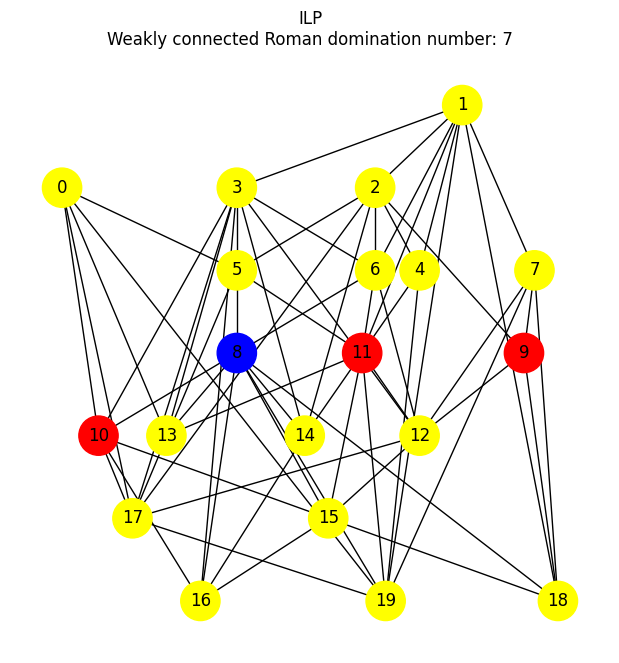
\includegraphics[width=0.75\linewidth]{assets/plots/ILP/ErdosRenyi_sparse_n20_i2_results.png}}
        \end{subcaptionbox}
        \hfill
        \begin{subcaptionbox}*{}[0.48\linewidth]
            {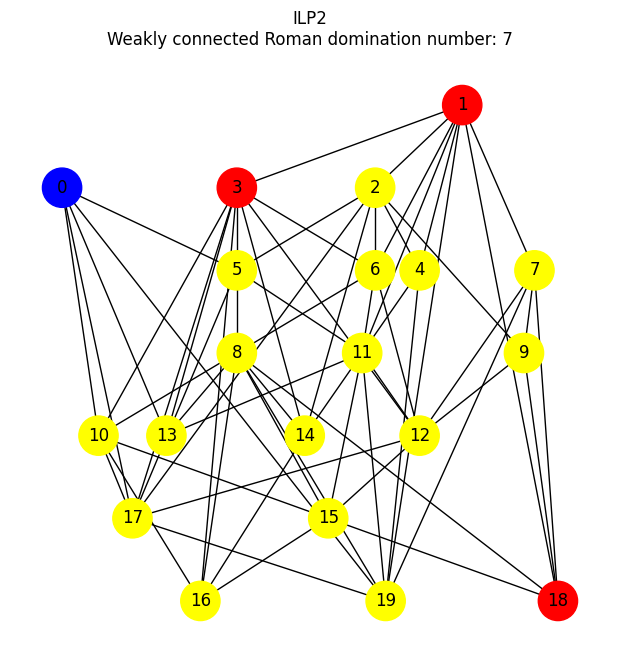
\includegraphics[width=0.75\linewidth]{assets/plots/ILP2/ErdosRenyi_sparse_n20_i2_results.png}}
        \end{subcaptionbox}
        \hfill
        \begin{subcaptionbox}*{}[0.48\linewidth]
            {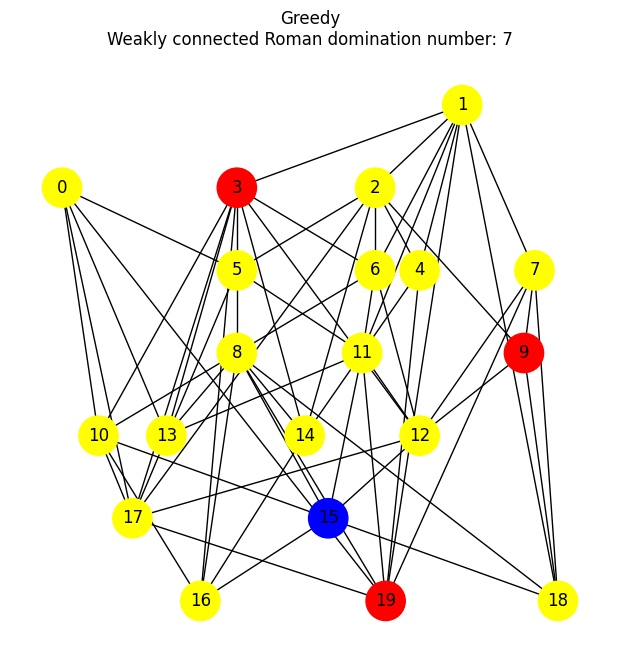
\includegraphics[width=0.75\linewidth]{assets/plots/Greedy/ErdosRenyi_sparse_n20_i2_results.png}}
        \end{subcaptionbox}
        \hfill
        \begin{subcaptionbox}*{}[0.48\linewidth]
            {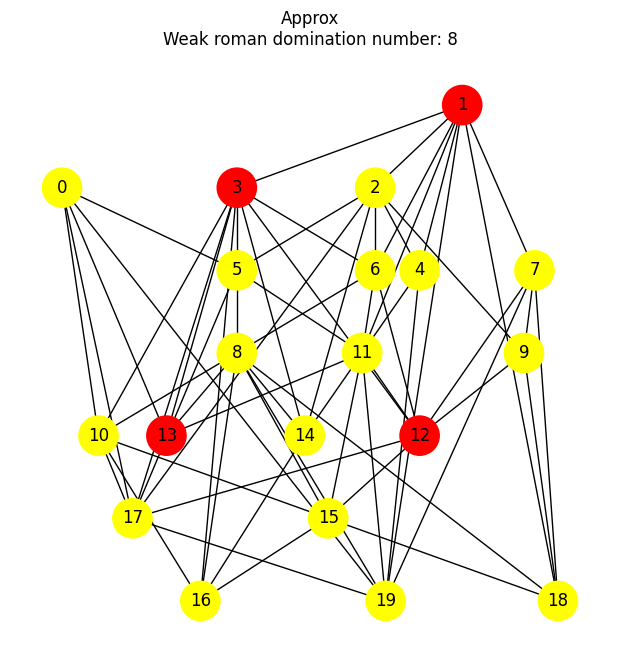
\includegraphics[width=0.75\linewidth]{assets/plots/Approx/ErdosRenyi_sparse_n20_i2_results.png}}
        \end{subcaptionbox}
        \hfill
        \begin{subcaptionbox}*{}[0.48\linewidth]
            {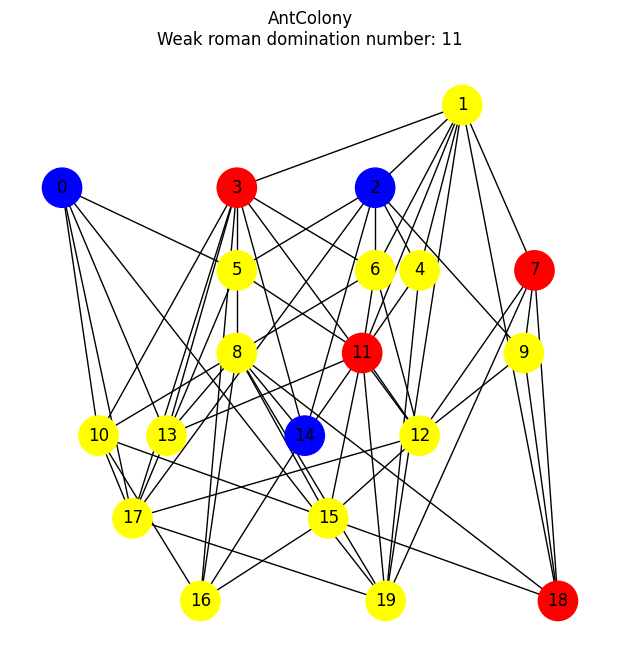
\includegraphics[width=0.75\linewidth]{assets/plots/AntColony/ErdosRenyi_sparse_n20_i2_results.png}}
        \end{subcaptionbox}
    
        \caption{Wyniki dla przykładowego grafu rzadkiego.}
        \label{fig:sparse}
    \end{figure}

    \begin{figure}[H]
        \centering
        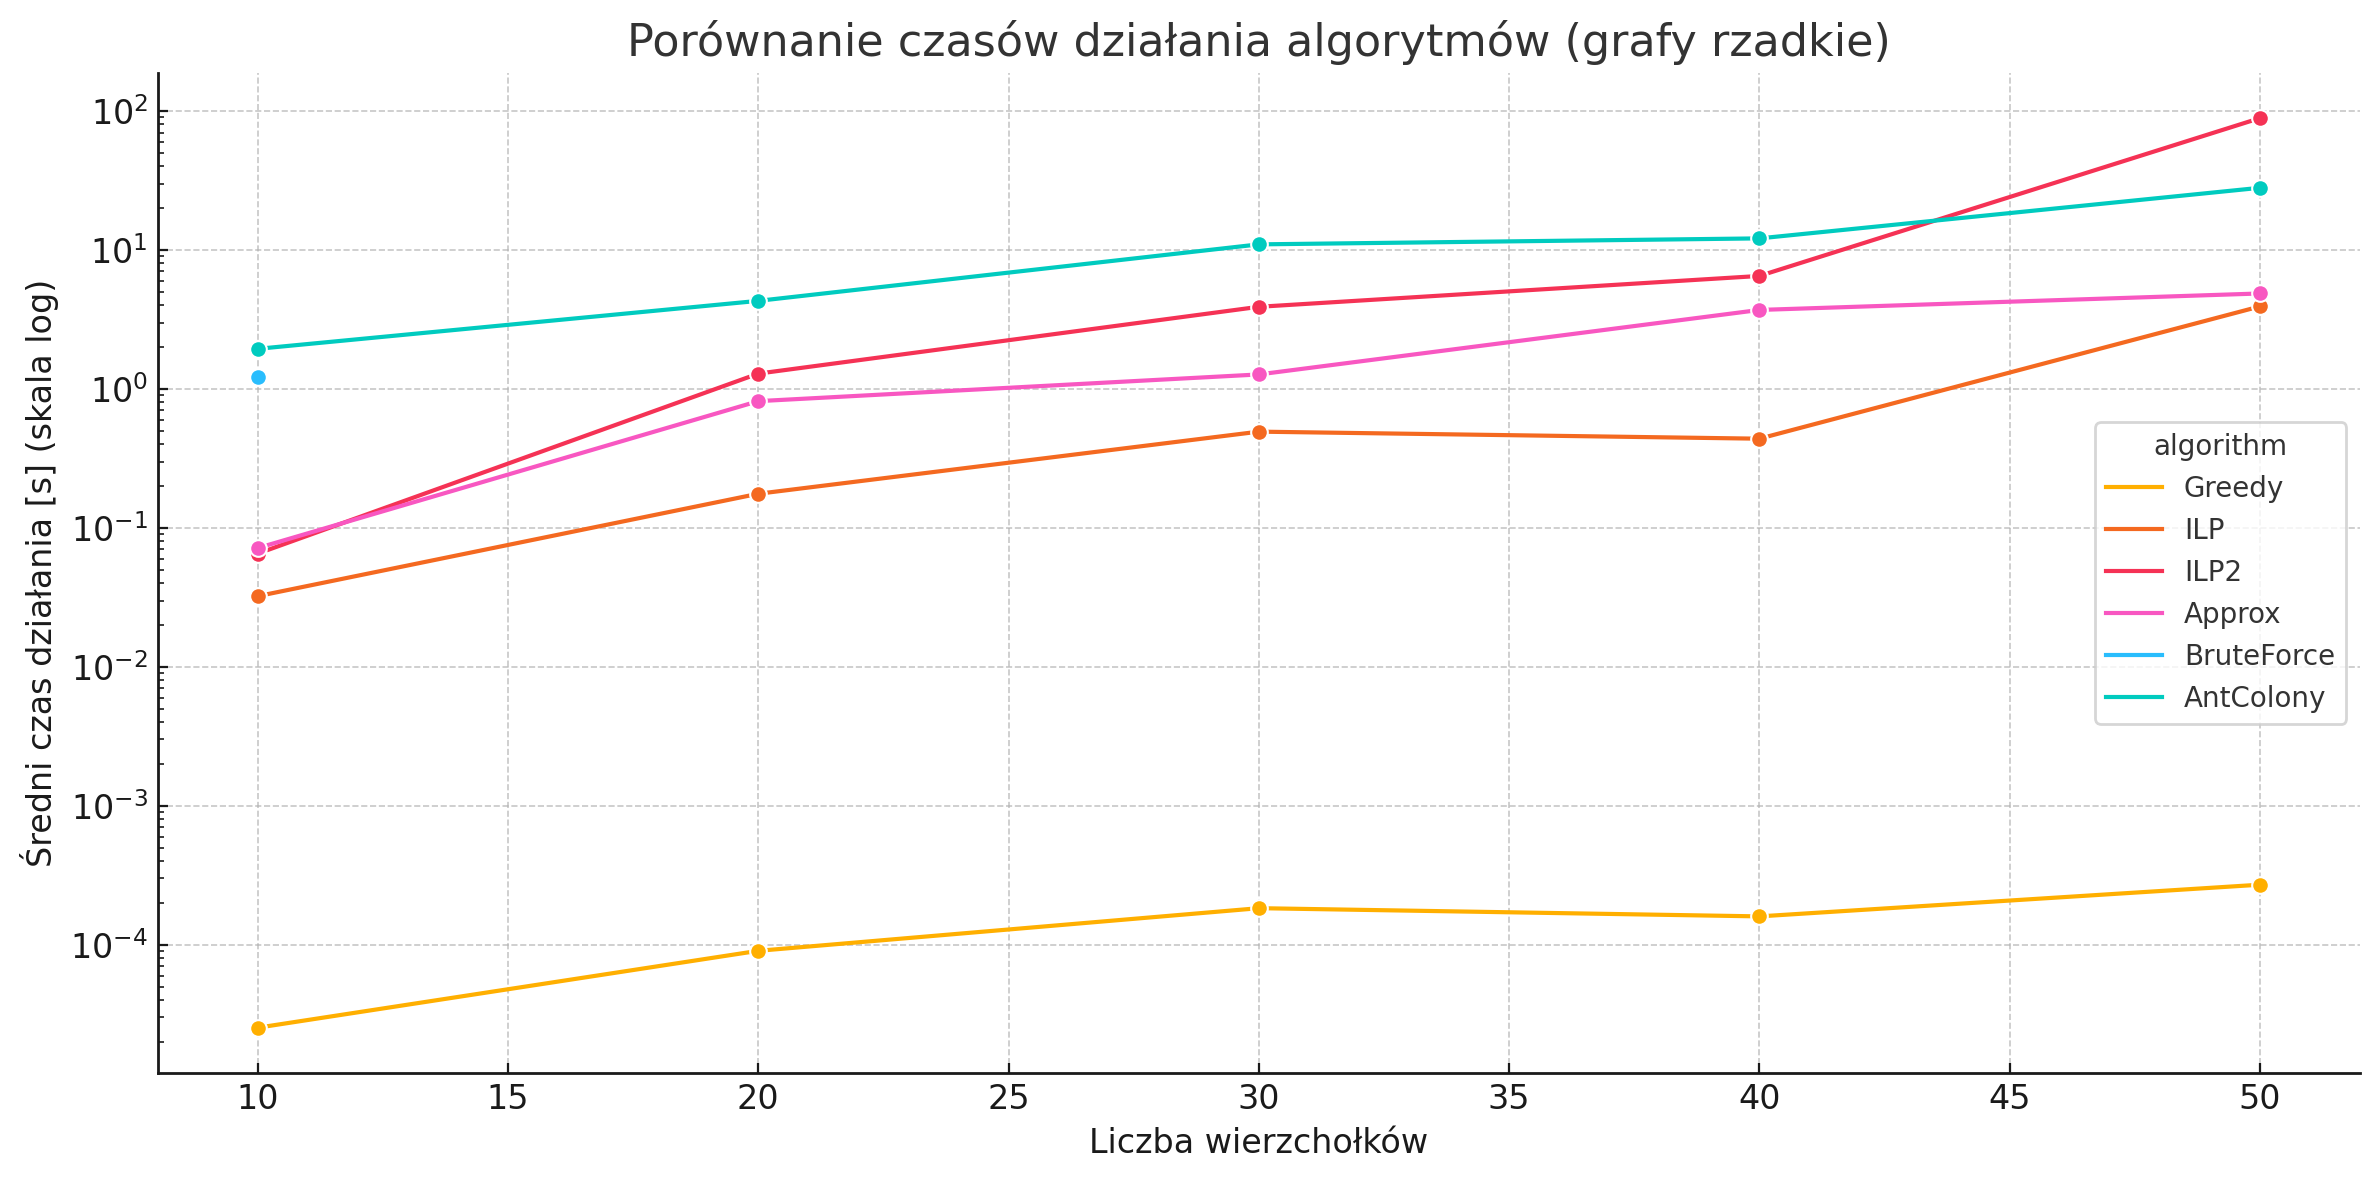
\includegraphics[width=\textwidth]{assets/sparse.png}
        \caption{Porównanie średniego czasu działania algorytmów na grafach rzadkich w stosunku do liczby wierzchołków w grafie.}
        \label{fig:sparsePlot}
    \end{figure}

\subsection{Grafy gęste}

\begin{table}[H]
    \centering
    \begin{tabular}{|c|c|c|c|c|}
    \hline
    Algorytm & Liczba wierzchołków & Liczba krawędzi & WCRDF & Średni czas (s) \\
    \hline
    Greedy & 10 & 31 & 2 & 0,00001534 \\
    ILP & 10 & 31 & 2 & 0,04773922 \\
    ILP2 & 10 & 31 & 2 & 0,06054642 \\
    Approx & 10 & 31 & 2 & 0,07325536 \\
    AntColony & 10 & 31 & 2 & 2,58175592 \\
    BruteForce & 10 & 31 & 2 & 3,39913678 \\
     \hline
     Greedy & 20 & 132 & 4 & 0,00011488 \\
     Approx & 20 & 132 & 4 & 0,17418222 \\
     ILP & 20 & 132 & 4 & 0,34445046 \\
     ILP2 & 20 & 132 & 4 & 1,10987306 \\
     AntColony & 20 & 132 & 9 & 11,15454742 \\
    \hline
    Greedy & 30 & 288 & 4 & 0,00006476 \\
    Approx & 30 & 288 & 4 & 0,22087496 \\
    ILP & 30 & 288 & 4 & 2,09136932 \\
    ILP2 & 30 & 288 & 4 & 2,7780365 \\
    AntColony & 30 & 288 & 14 & 15,7567997 \\
    \hline
    Greedy & 40 & 522 & 5 & 0,0001943 \\
    Approx & 40 & 522 & 4 & 0,32690006 \\
    ILP2 & 40 & 522 & 4 & 16,49655814 \\
    AntColony & 40 & 522 & 21 & 29,47564454 \\
    ILP & 40 & 522 & 4 & 77,93719362 \\
    \hline
    Greedy & 50 & 839 & 5 & 0,00027366 \\
    Approx & 50 & 839 & 4 & 0,45039484 \\
    AntColony & 50 & 839 & 28 & 45,90004724 \\
    ILP2 & 50 & 839 & 4 & 345,33312052 \\
    ILP & 50 & 839 & 4 & 690,41462788 \\

    \hline
    \end{tabular}
    \caption{Wyniki dla grafów gęstych}
    \end{table}

    \begin{figure}[H]
        \centering
        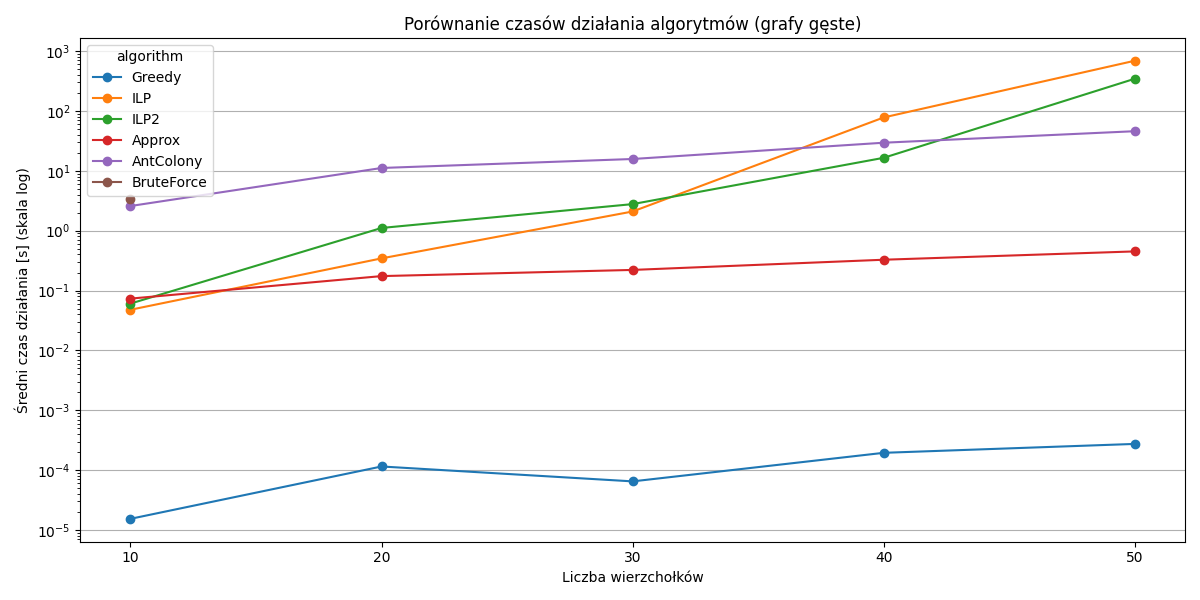
\includegraphics[width=\textwidth]{assets/dense.png}
        \caption{Porównanie średniego czasu działania algorytmów na grafach gęstych w stosunku do liczby wierzchołków w grafie.}
        \label{fig:densePlot}
    \end{figure}

    \begin{figure}[htbp]
        \centering
        \begin{subcaptionbox}*{}[0.48\linewidth]
            {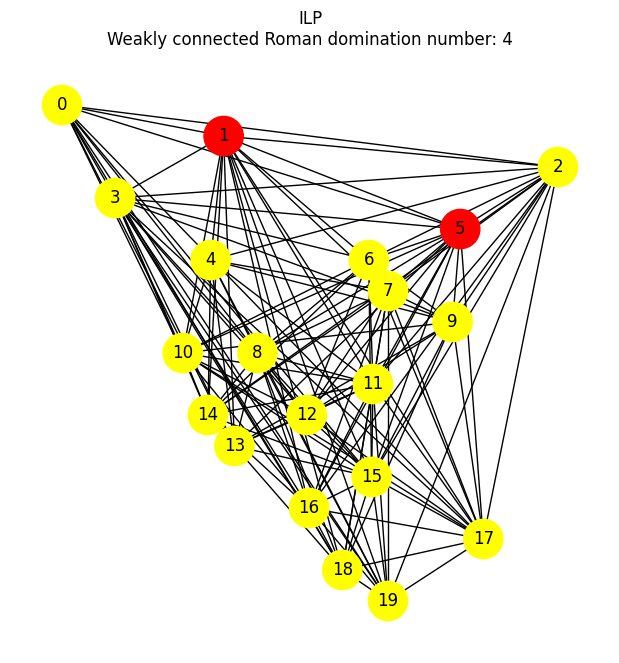
\includegraphics[width=0.75\linewidth]{assets/plots/ILP/ErdosRenyi_dense_n20_i2_results.png}}
        \end{subcaptionbox}
        \hfill
        \begin{subcaptionbox}*{}[0.48\linewidth]
            {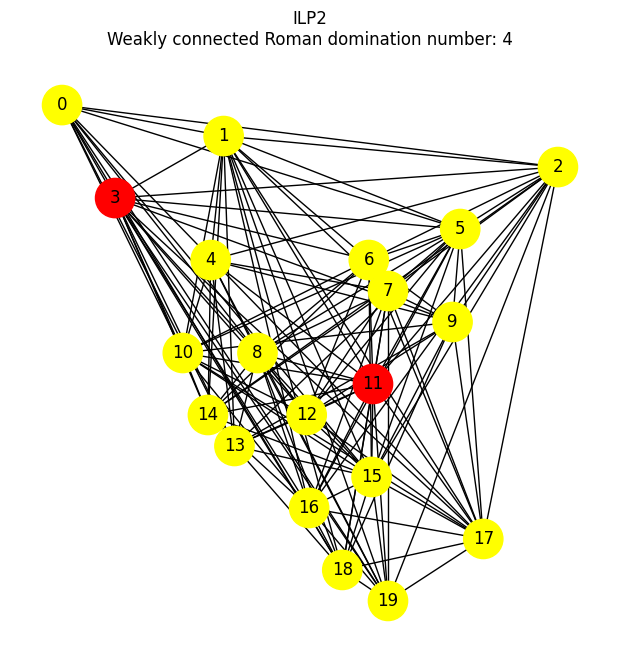
\includegraphics[width=0.75\linewidth]{assets/plots/ILP2/ErdosRenyi_dense_n20_i2_results.png}}
        \end{subcaptionbox}
        \hfill
        \begin{subcaptionbox}*{}[0.48\linewidth]
            {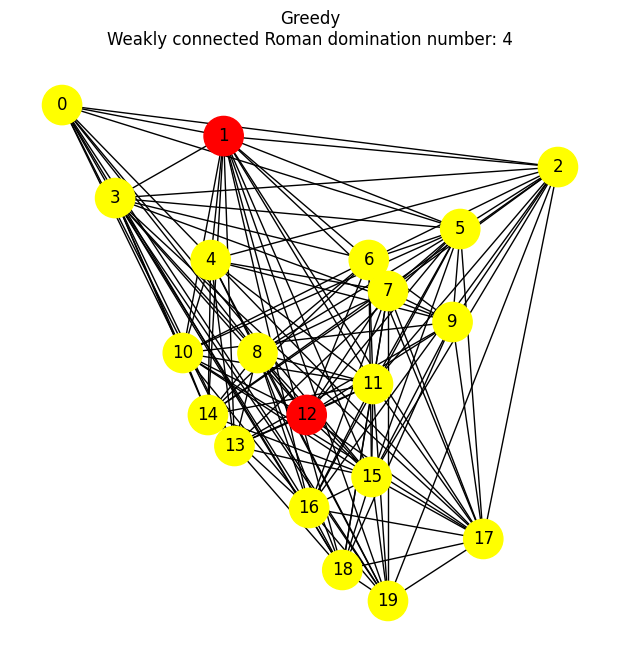
\includegraphics[width=0.75\linewidth]{assets/plots/Greedy/ErdosRenyi_dense_n20_i2_results.png}}
        \end{subcaptionbox}
        \hfill
        \begin{subcaptionbox}*{}[0.48\linewidth]
            {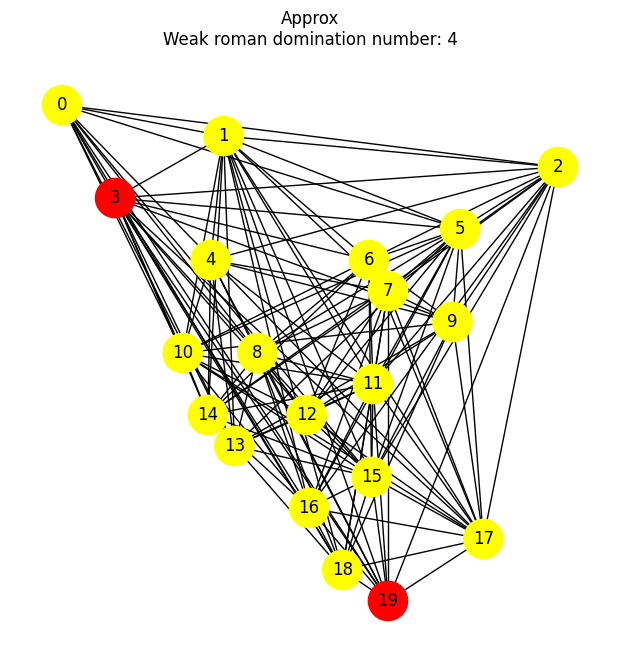
\includegraphics[width=0.75\linewidth]{assets/plots/Approx/ErdosRenyi_dense_n20_i2_results.png}}
        \end{subcaptionbox}
        \hfill
        \begin{subcaptionbox}*{}[0.48\linewidth]
            {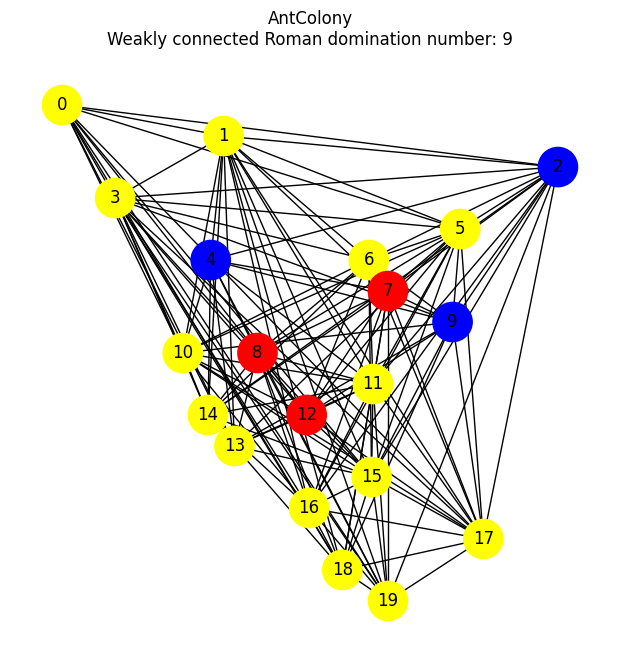
\includegraphics[width=0.75\linewidth]{assets/plots/AntColony/ErdosRenyi_dense_n20_i2_results.png}}
        \end{subcaptionbox}
    
        \caption{Wyniki dla przykładowego grafu gęstego.}
        \label{fig:dense}
    \end{figure}

\subsection{Drzewa}

\begin{table}[H]
    \centering
    \begin{tabular}{|c|c|c|c|c|}
    \hline
    Algorytm & Liczba wierzchołków & Liczba krawędzi & WCRDF & Średni czas (s) \\
    \hline
    Greedy & 10 & 9 & 8 & 0,00005232 \\
    TreeLinear & 10 & 9 & 7 & 0,00051616 \\
    ILP & 10 & 9 & 7 & 0,04267752 \\
    ILP2 & 10 & 9 & 7 & 0,04535534 \\
    Approx & 10 & 9 & 14 & 0,3153601 \\
    BruteForce & 10 & 9 & 7 & 0,65010432 \\
    AntColony & 10 & 9 & 8 & 1,19096304 \\
    \hline
    Greedy & 20 & 19 & 12 & 0,00007772 \\
    TreeLinear & 20 & 19 & 12 & 0,00089554 \\
    ILP & 20 & 19 & 12 & 0,04966132 \\
    ILP2 & 20 & 19 & 12 & 0,07429058 \\
    Approx & 20 & 19 & 16 & 0,20606074 \\
    AntColony & 20 & 19 & 18 & 2,04032124 \\
    \hline
    Greedy & 30 & 29 & 20 & 0,0001205 \\
    TreeLinear & 30 & 29 & 17 & 0,00148292 \\
    ILP & 30 & 29 & 17 & 0,04517938 \\
    ILP2 & 30 & 29 & 17 & 0,13887008 \\
    Approx & 30 & 29 & 36 & 1,0127093 \\
    AntColony & 30 & 29 & 30 & 4,13727904 \\
     \hline
     Greedy & 40 & 39 & 33 & 0,00021536 \\
     TreeLinear & 40 & 39 & 29 & 0,0017755 \\
     ILP & 40 & 39 & 29 & 0,06708872 \\
     ILP2 & 40 & 39 & 29 & 0,48569172 \\
     Approx & 40 & 39 & 48 & 3,7790714 \\
     AntColony & 40 & 39 & 43 & 3,79114808 \\
    \hline
    Greedy & 50 & 49 & 45 & 0,00107456 \\
    TreeLinear & 50 & 49 & 35 & 0,00480282 \\
    ILP & 50 & 49 & 35 & 0,07759686 \\
    ILP2 & 50 & 49 & 35 & 0,82981668 \\
    Approx & 50 & 49 & 66 & 5,0276923 \\
    AntColony & 50 & 49 & 59 & 12,4118761 \\ 
    \hline
    \end{tabular}
    \caption{Wyniki dla drzew}
    \end{table}

    \begin{figure}[H]
        \centering
        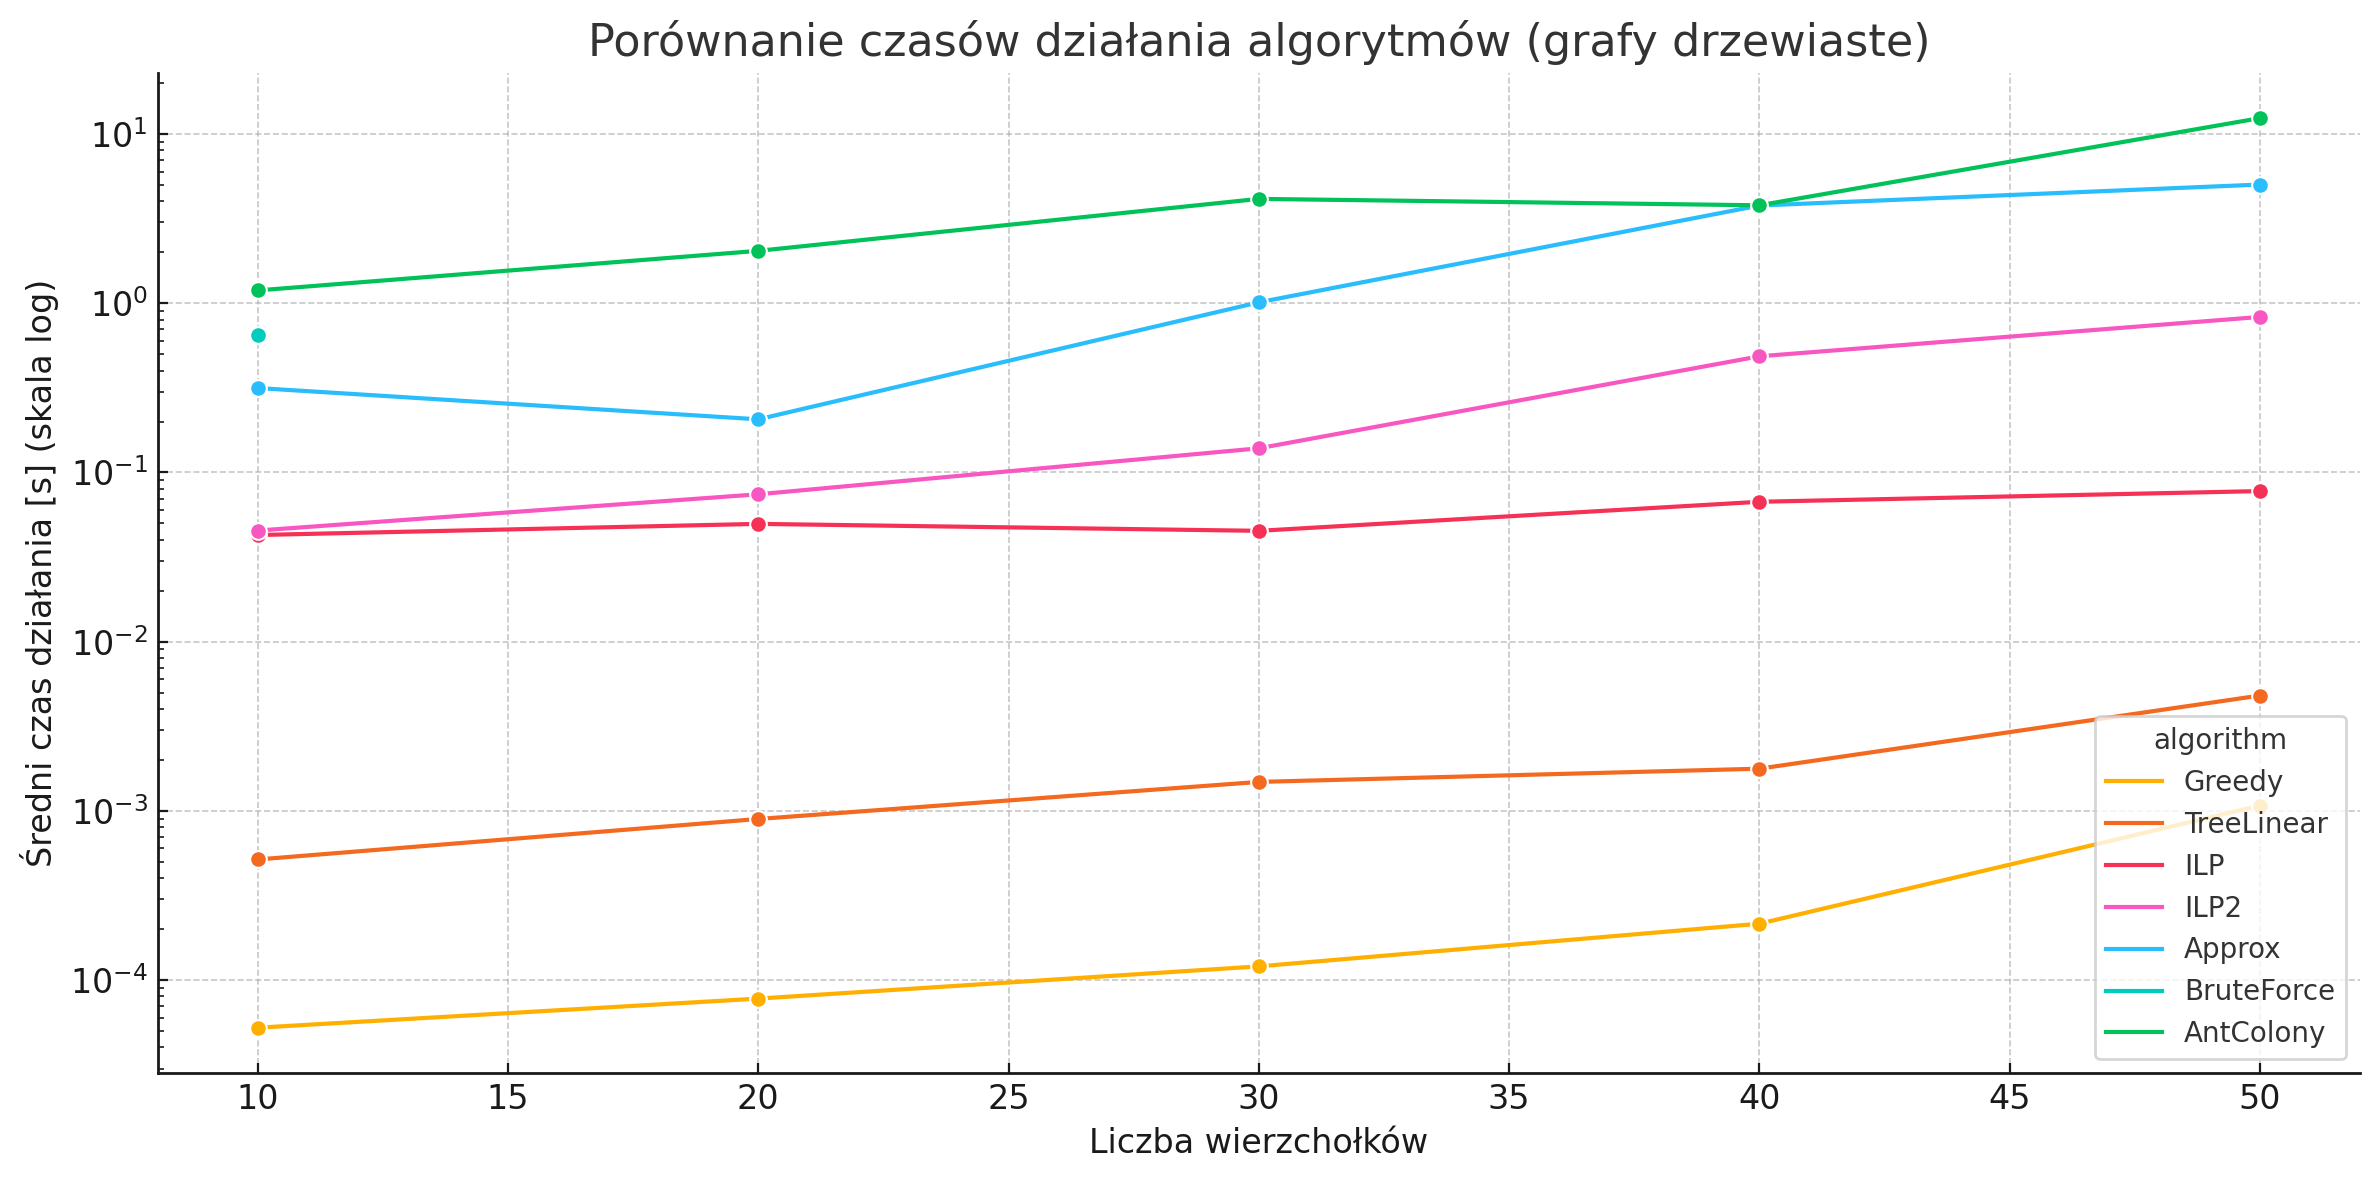
\includegraphics[width=\textwidth]{assets/trees.png}
        \caption{Porównanie średniego czasu działania algorytmów na drzewach w stosunku do liczby wierzchołków w grafie.}
        \label{fig:treePlot}
    \end{figure}

    \begin{figure}[htbp]
        \centering
        \begin{subcaptionbox}*{}[0.48\linewidth]
            {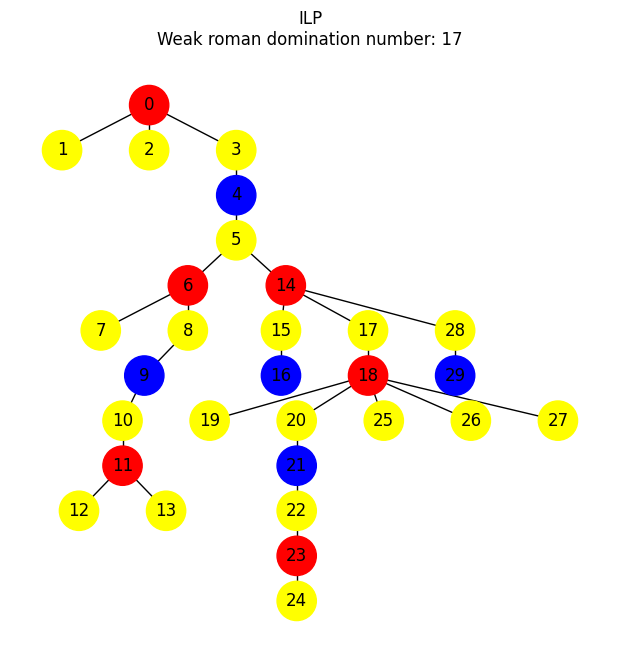
\includegraphics[width=0.75\linewidth]{assets/plots/ILP/RandomTree_n30_i2_results.png}}
        \end{subcaptionbox}
        \hfill
        \begin{subcaptionbox}*{}[0.48\linewidth]
            {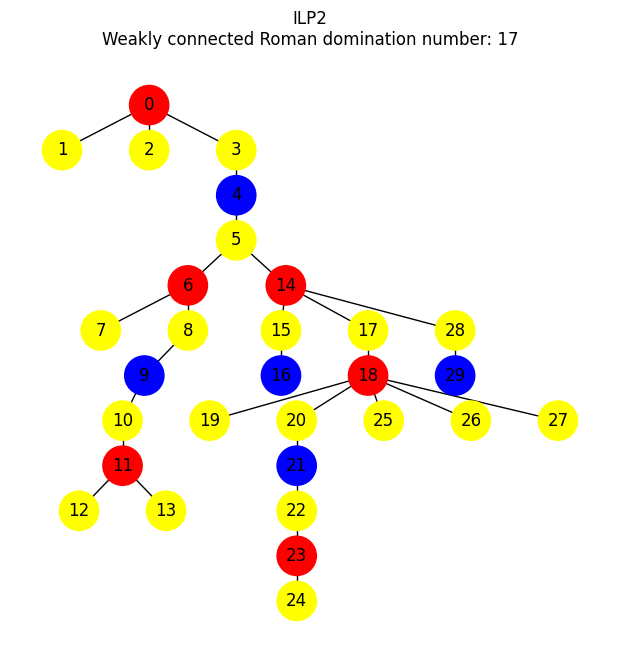
\includegraphics[width=0.75\linewidth]{assets/plots/ILP2/RandomTree_n30_i2_results.png}}
        \end{subcaptionbox}
        \hfill
        \begin{subcaptionbox}*{}[0.48\linewidth]
            {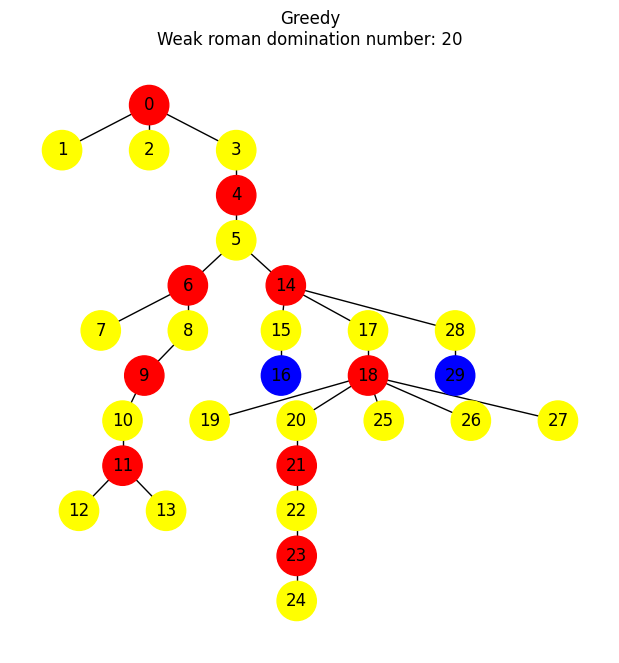
\includegraphics[width=0.75\linewidth]{assets/plots/Greedy/RandomTree_n30_i2_results.png}}
        \end{subcaptionbox}
        \hfill
        \begin{subcaptionbox}*{}[0.48\linewidth]
            {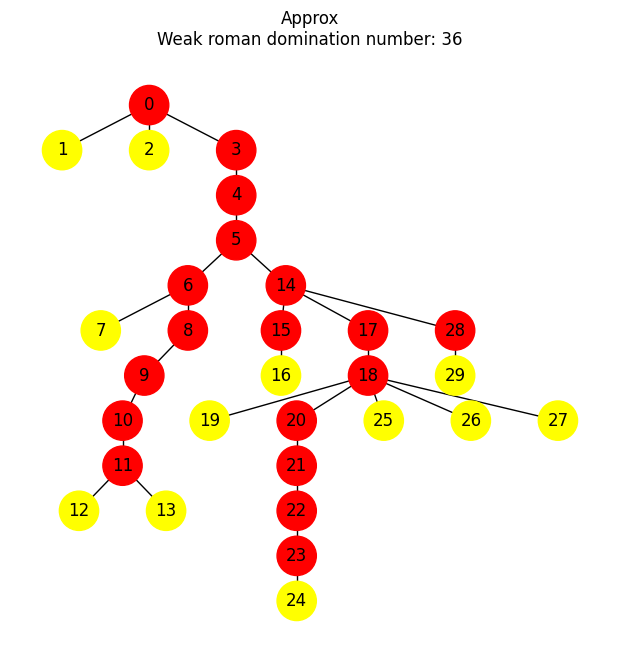
\includegraphics[width=0.75\linewidth]{assets/plots/Approx/RandomTree_n30_i2_results.png}}
        \end{subcaptionbox}
        \hfill
        \begin{subcaptionbox}*{}[0.48\linewidth]
            {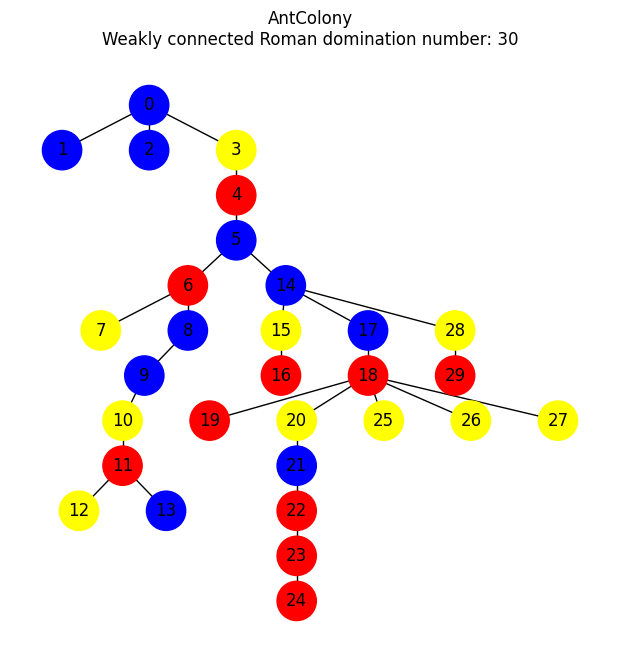
\includegraphics[width=0.75\linewidth]{assets/plots/AntColony/RandomTree_n30_i2_results.png}}
        \end{subcaptionbox}
        \hfill
        \begin{subcaptionbox}*{}[0.48\linewidth]
            {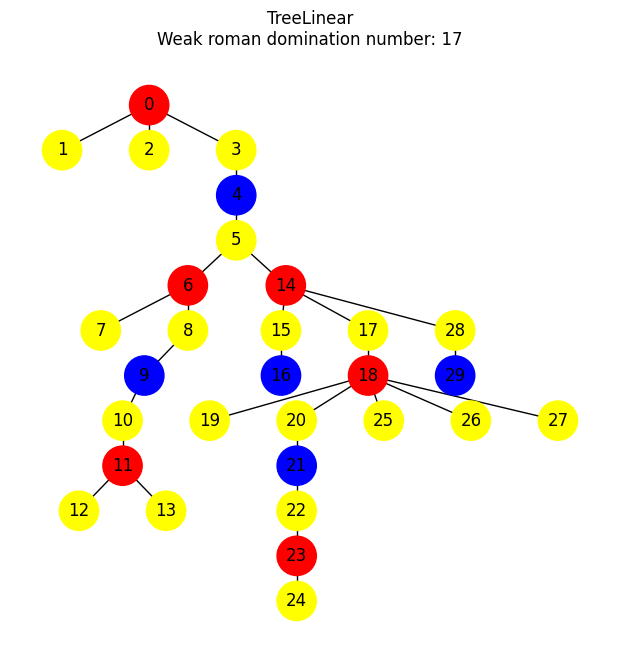
\includegraphics[width=0.75\linewidth]{assets/plots/TreeLinear/RandomTree_n30_i2_results.png}}
        \end{subcaptionbox}
    
        \caption{Wyniki dla przykładowego drzewa.}
        \label{fig:tree}
    \end{figure}


\subsection{Grafy bezskalowe}

\begin{table}[H]
    \centering
    \begin{tabular}{|c|c|c|c|c|}
    \hline
    Algorytm & Liczba wierzchołków & Liczba krawędzi & WCRDF & Średni czas (s) \\
    \hline
    Greedy & 10 & 25 & 2 & 0,00001166 \\
    ILP & 10 & 25 & 2 & 0,04384846 \\
    ILP2 & 10 & 25 & 2 & 0,05840188 \\
    Approx & 10 & 25 & 2 & 0,06902438 \\
    BruteForce & 10 & 25 & 2 & 2,3746041 \\
    AntColony & 10 & 25 & 3 & 3,02645522 \\
     \hline
     Greedy & 20 & 75 & 5 & 0,00008788 \\
     ILP & 20 & 75 & 4 & 0,1319412 \\
     Approx & 20 & 75 & 4 & 0,13767914 \\
     ILP2 & 20 & 75 & 4 & 0,25321824 \\
     AntColony & 20 & 75 & 9 & 8,82321618 \\ 
    \hline
    Greedy & 30 & 125 & 9 & 0,00009044 \\
    ILP & 30 & 125 & 6 & 0,08527778 \\
    ILP2 & 30 & 125 & 6 & 0,15141182 \\
    Approx & 30 & 125 & 6 & 0,16305526 \\
    AntColony & 30 & 125 & 18 & 10,0423744 \\ 
    \hline
    Greedy & 40 & 175 & 10 & 0,00026662 \\
    ILP & 40 & 175 & 7 & 0,1015079 \\
    Approx & 40 & 175 & 8 & 0,18101464 \\
    ILP2 & 40 & 175 & 7 & 0,3487031 \\
    AntColony & 40 & 175 & 24 & 9,48435894 \\
    \hline
    Greedy & 50 & 225 & 14 & 0,00024856 \\
    Approx & 50 & 225 & 10 & 0,17308662 \\
    ILP & 50 & 225 & 10 & 0,48920074 \\
    ILP2 & 50 & 225 & 10 & 0,82045656 \\
    AntColony & 50 & 225 & 35 & 20,21980648 \\
    
    \hline
    \end{tabular}
    \caption{Wyniki dla grafów bezskalowych}
    \end{table}

    \begin{figure}[H]
        \centering
        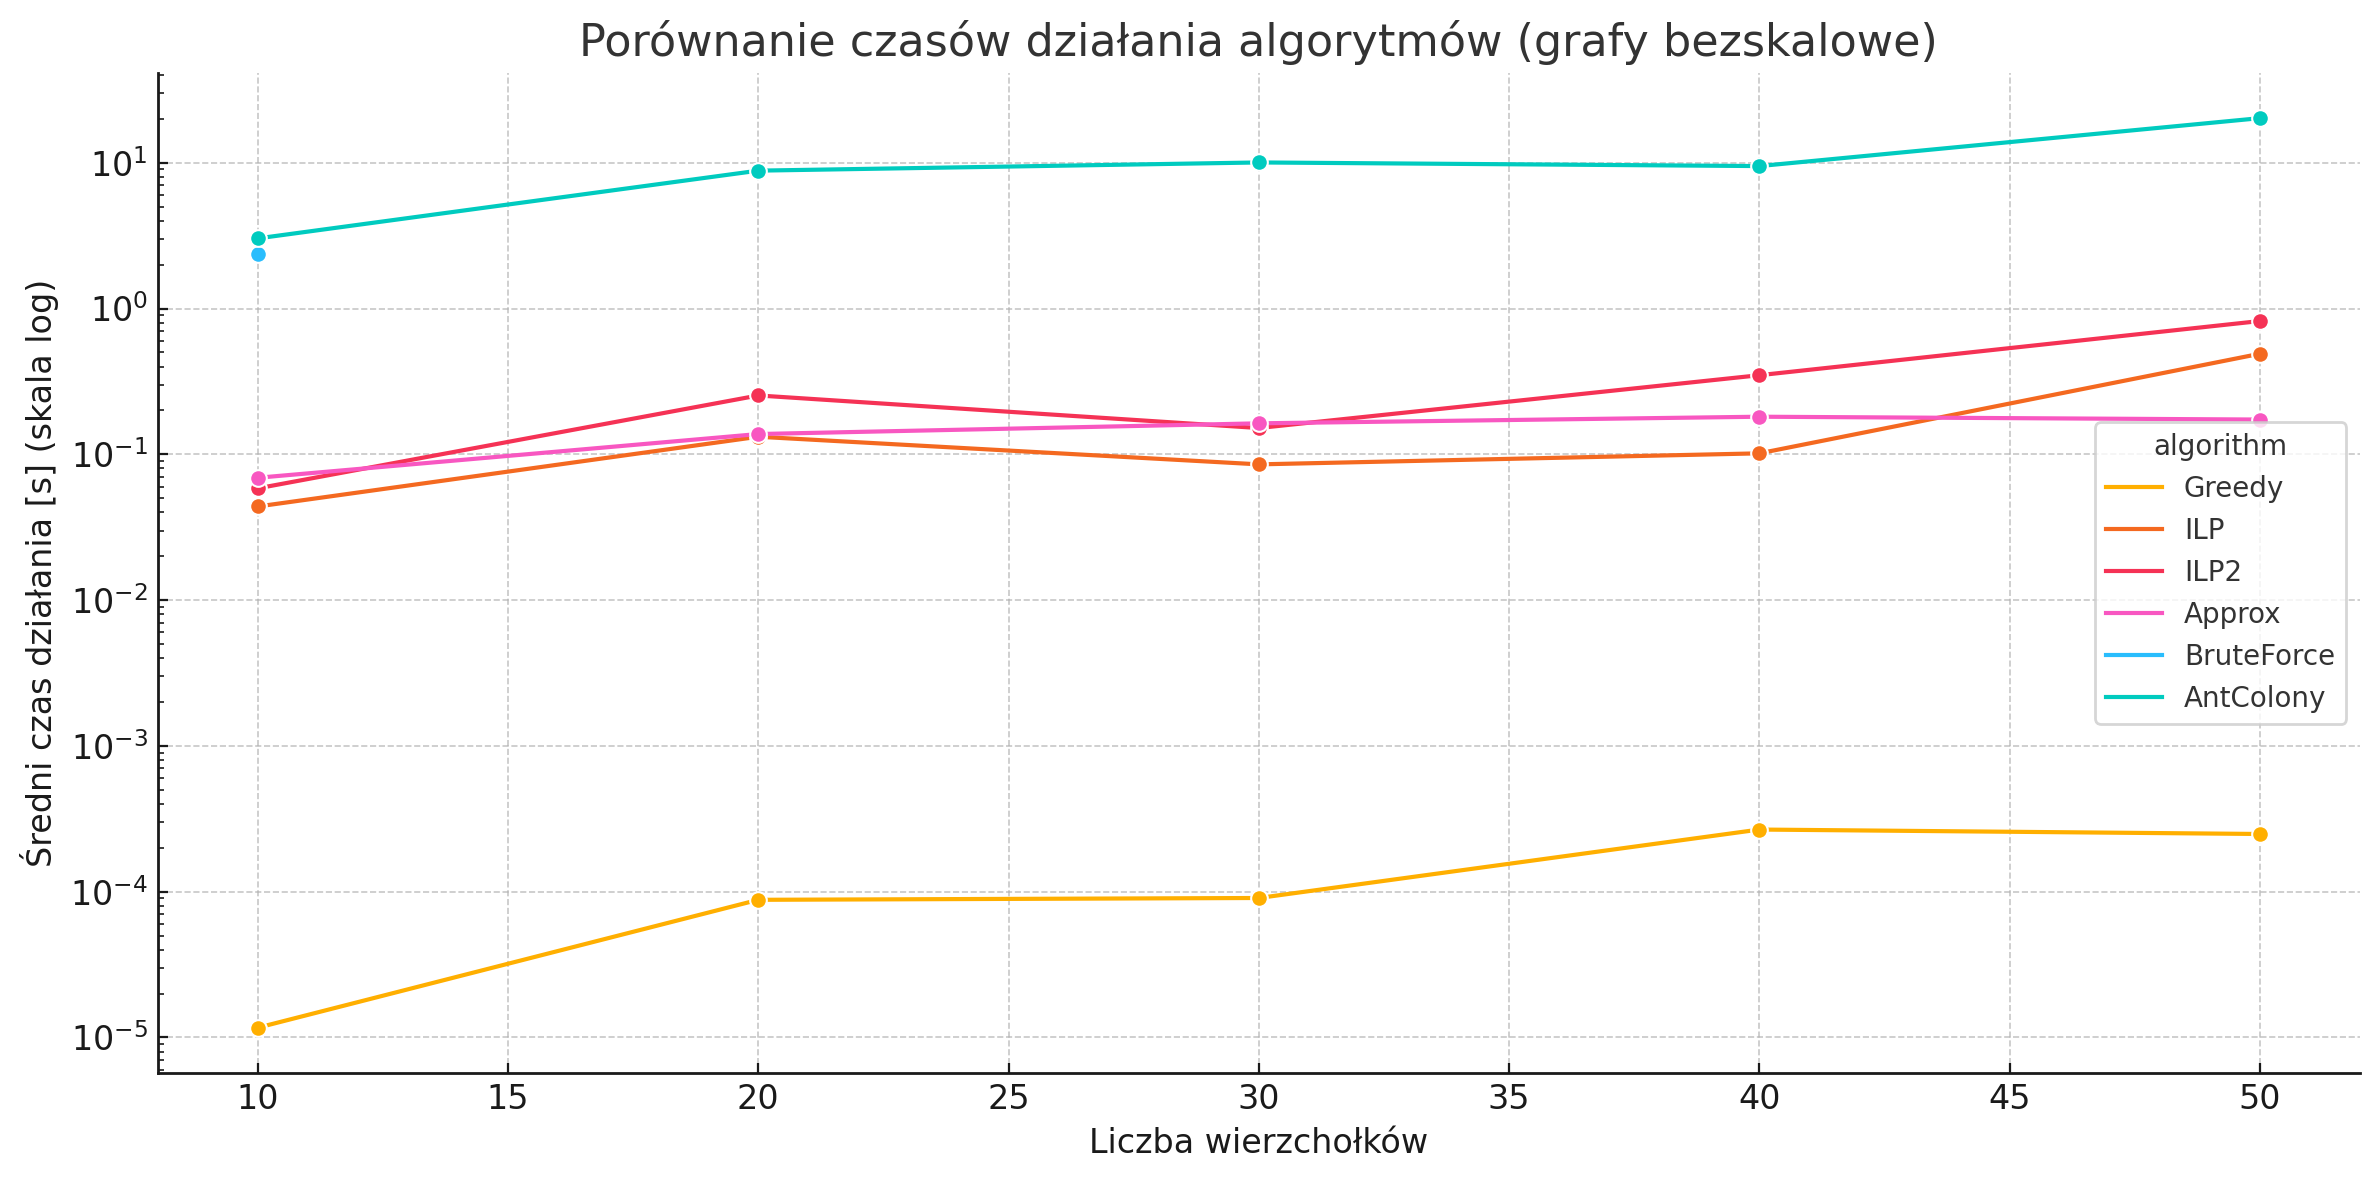
\includegraphics[width=\textwidth]{assets/scaleFree.png}
        \caption{Porównanie średniego czasu działania algorytmów na grafach bezskalowych w stosunku do liczby wierzchołków w grafie.}
        \label{fig:scaleFreePlot}
    \end{figure}

    \begin{figure}[htbp]
        \centering
        \begin{subcaptionbox}*{}[0.48\linewidth]
            {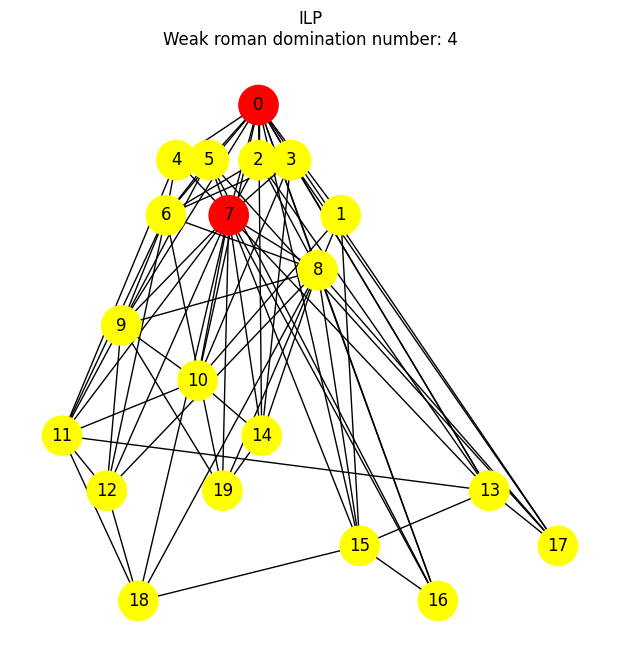
\includegraphics[width=0.75\linewidth]{assets/plots/ILP/ScaleFree_n20_i2_results.png}}
        \end{subcaptionbox}
        \hfill
        \begin{subcaptionbox}*{}[0.48\linewidth]
            {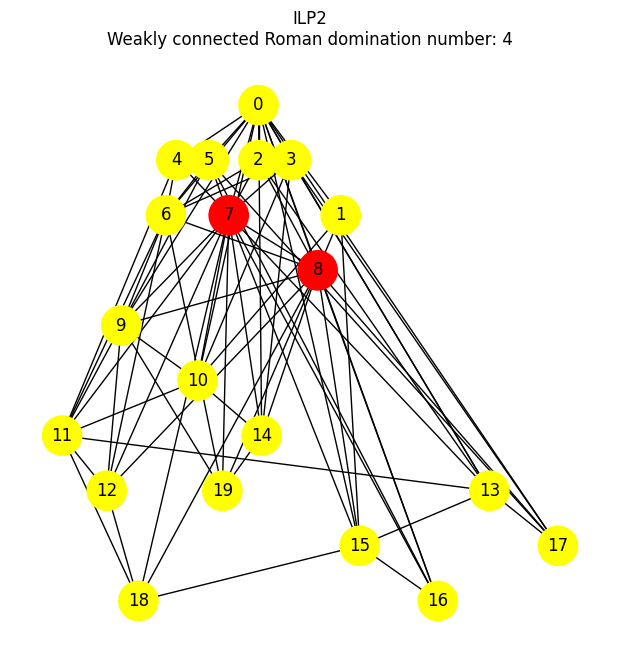
\includegraphics[width=0.75\linewidth]{assets/plots/ILP2/ScaleFree_n20_i2_results.png}}
        \end{subcaptionbox}
        \hfill
        \begin{subcaptionbox}*{}[0.48\linewidth]
            {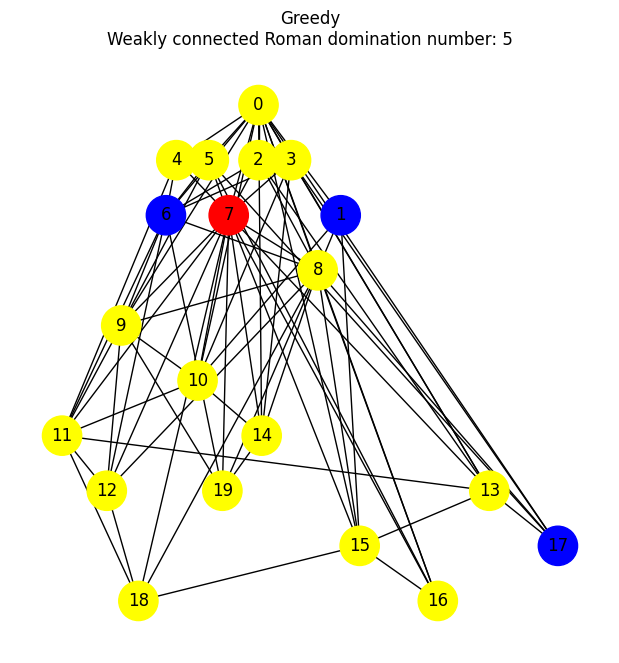
\includegraphics[width=0.75\linewidth]{assets/plots/Greedy/ScaleFree_n20_i2_results.png}}
        \end{subcaptionbox}
        \hfill
        \begin{subcaptionbox}*{}[0.48\linewidth]
            {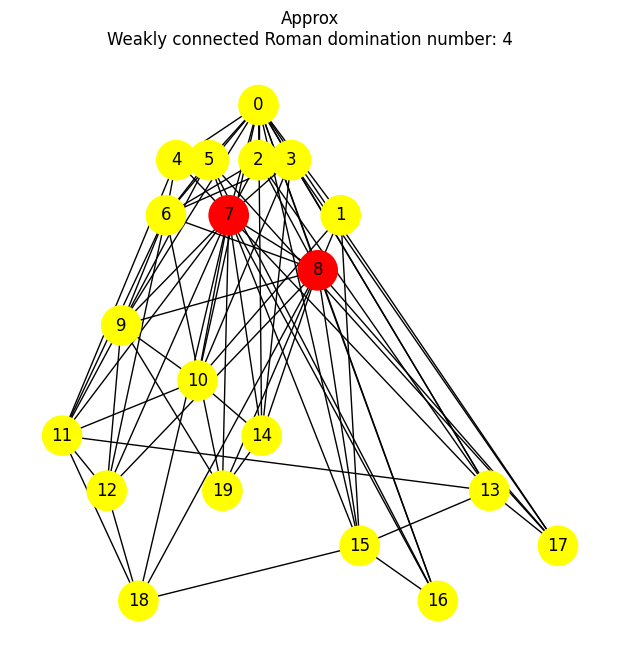
\includegraphics[width=0.75\linewidth]{assets/plots/Approx/ScaleFree_n20_i2_results.png}}
        \end{subcaptionbox}
        \hfill
        \begin{subcaptionbox}*{}[0.48\linewidth]
            {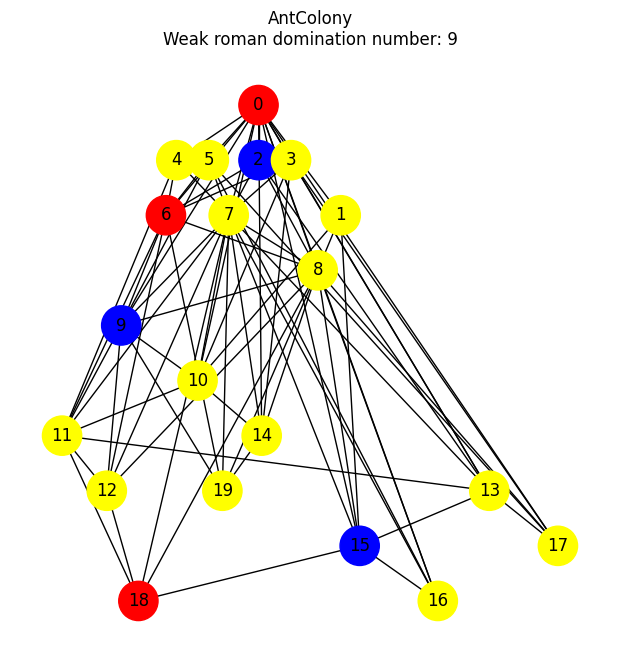
\includegraphics[width=0.75\linewidth]{assets/plots/AntColony/ScaleFree_n20_i2_results.png}}
        \end{subcaptionbox}
    
        \caption{Wyniki dla przykładowego grafu bezskalowego.}
        \label{fig:tree}
    \end{figure}

\section{Wyniki algorytmów niedokładnych}

\subsection{Algorytm mrówkowy}

\begin{figure}[H]
    \centering
    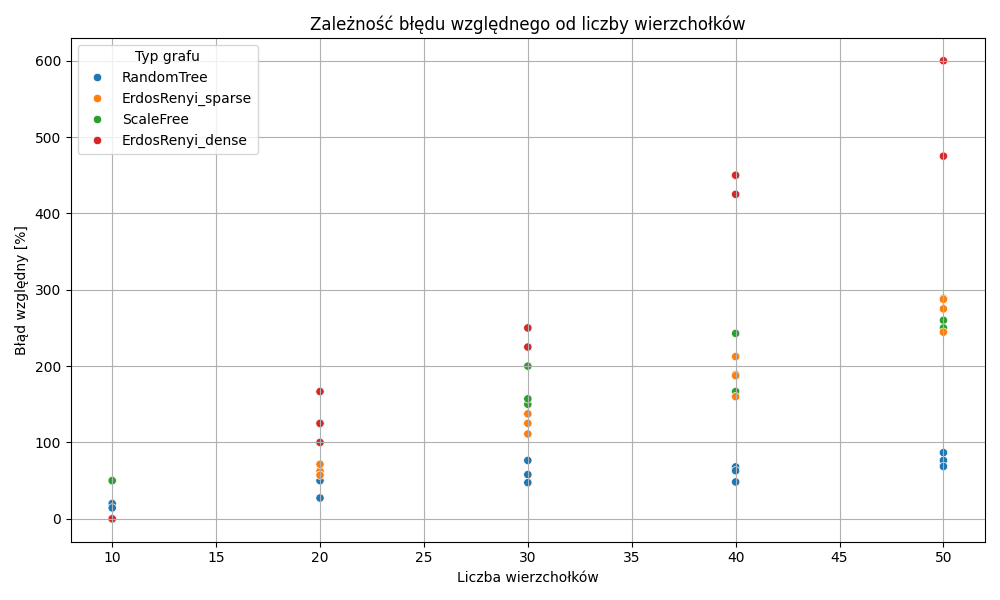
\includegraphics[width=\textwidth]{assets/plots_approx/ants.png}
    \caption{Zależność błędu względnego algorytmu mrówkowego od liczby wierzchołków.}
    \label{fig:antsPlot}
\end{figure}

\subsection{Algorytm zachłanny}

\begin{figure}[H]
    \centering
    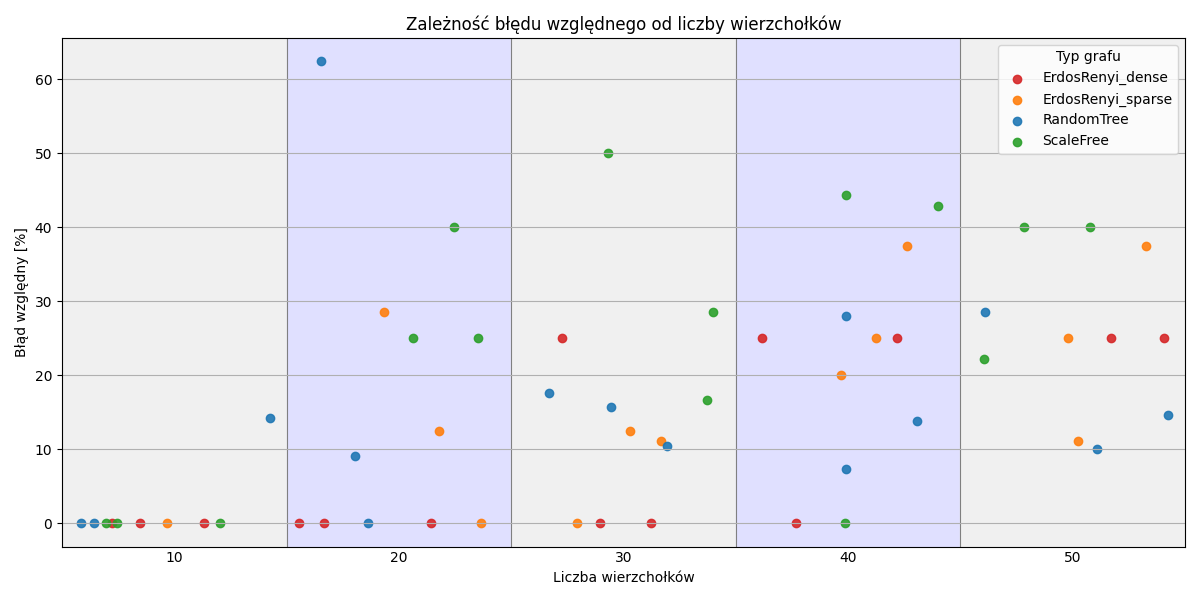
\includegraphics[width=\textwidth]{assets/plots_approx/greedy.png}
    \caption{Zależność błędu względnego algorytmu zachłannego od liczby wierzchołków.}
    \label{fig:greedyPlot}
\end{figure}

\subsection{Algorytm aproksymacyjny}

\begin{figure}[H]
    \centering
    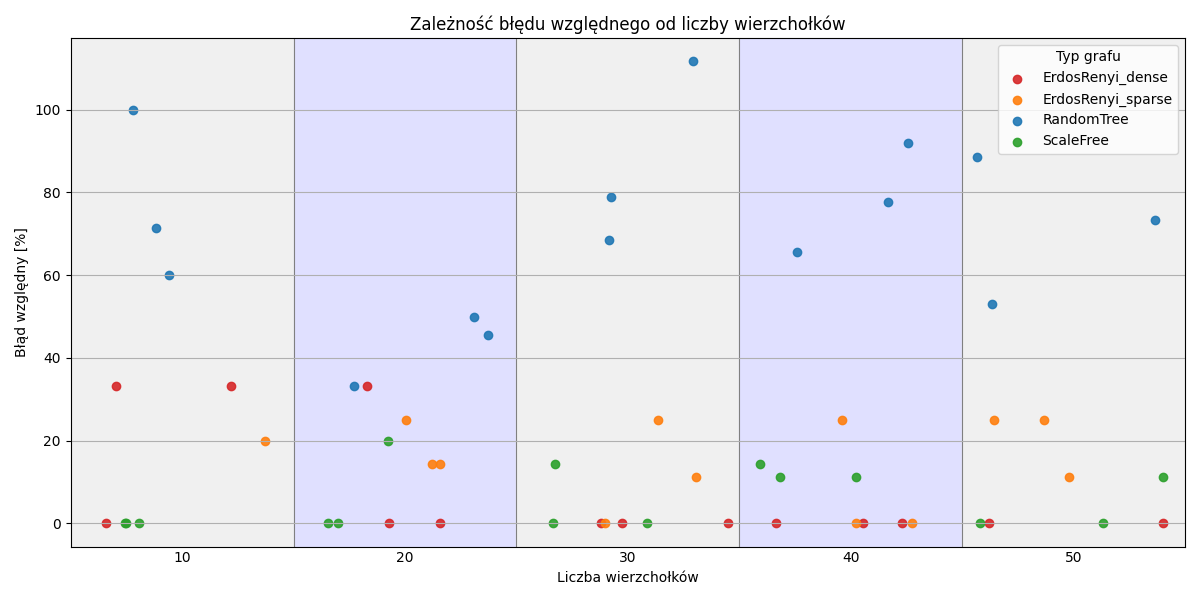
\includegraphics[width=\textwidth]{assets/plots_approx/approx.png}
    \caption{Zależność błędu względnego algorytmu aproksymacyjnego od liczby wierzchołków.}
    \label{fig:approxPlot}
\end{figure}

\begin{figure}[H]
    \centering
    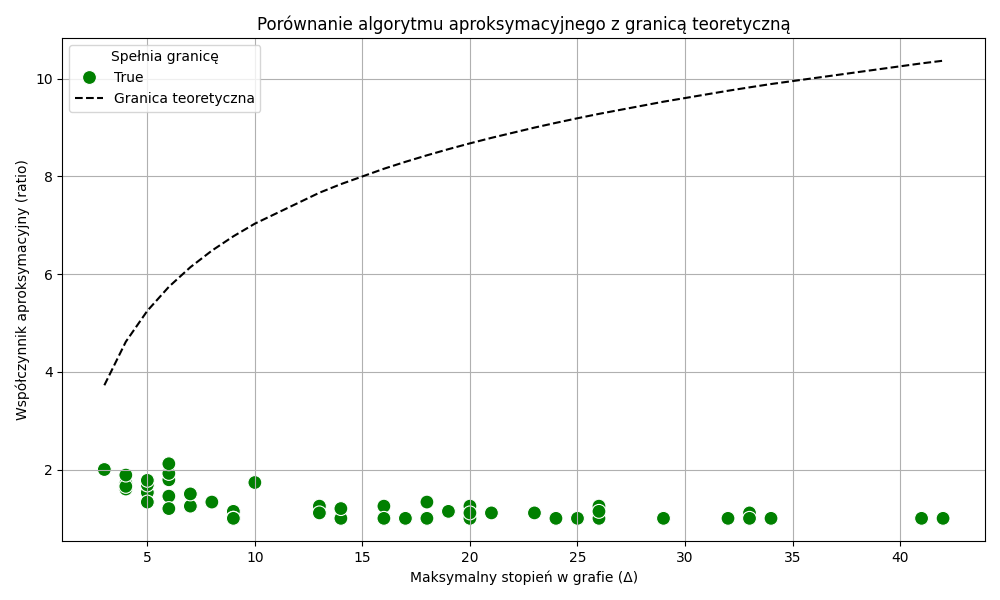
\includegraphics[width=\textwidth]{assets/plots_approx/image.png}
    \caption{Porównanie algorytmu aproksymacyjnego z granicą teoretyczną $2(1+\epsilon)(1 + \ln(\Delta - 1))$.}
    \label{fig:approxPlot}
\end{figure}

\subsection{Porównanie algorytmów przybliżonych}

\begin{figure}[H]
    \centering
    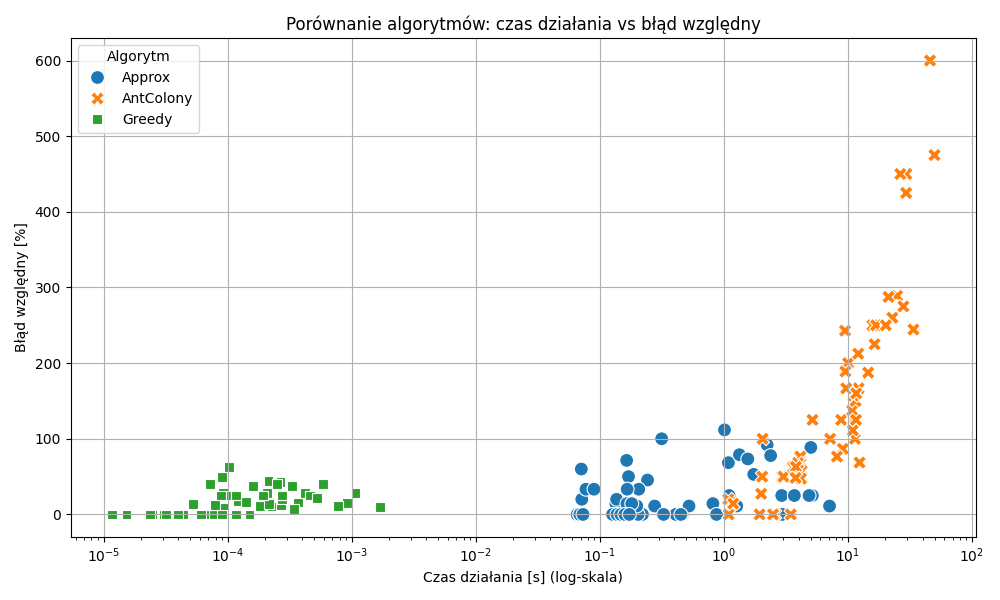
\includegraphics[width=\textwidth]{assets/plots_approx/alorithms.png}
    \caption{Algorytmy przybliżone: czas działania w stosunku do błędu względnego.}
    \label{fig:approxPlot}
\end{figure}

